\newpage
\topskip0pt
\vspace*{\fill}
\section*{Abstract}
Determining the size and structure of nature reserves that are best suited to preserving biodiversity and abundance is an important question for conservation, although it has received little theoretical attention. We examine the effects of introducing protected reserves where disturbance pressure is removed, and investigate the effects of varying the size of these reserves, by expanding the model presented in Chapter~2 to include both additional species and a metapopulation structure. We find that spatial heterogeneity in disturbance pressure is necessary to support $n>2$ species in a community, while protected reserves are most likely to increase $\gamma$ diversity when they are smaller. We observe no relationship between reserve size and within-reserve $\alpha$ diversity, although when reserves are small, an increase in species richness in the neighbouring, unprotected area is observed.
\vspace*{\fill}
\newpage
\section{Introduction}
Studies have suggested that disturbance, caused by either natural or anthropogenic events, play an important role in maintaining high levels of species richness in a community \citep{connell1978diversity,huston1979general,sousa1984role,schoener1974resource}. Most commonly, the case where the ability to colonise an empty habitat is traded off against local competitiveness is considered \citep[e.g.][]{tilman1994competition, cadotte2006testing}. In a constant environment, the poorer local competitor will be excluded, yet disturbance events can enable the persistence of this poor competitor in the community by creating empty habitat. Then, the greater colonising ability of the poor competitor enables long term survival \citep{sousa1984role,denslow1987tropical,connell1978diversity,grime1973competitive,huston1979general}. It has been argued that there are at least three main axes upon which disturbance should be measured \cite{malanson1984intensity,miller1982community,sousa1984role}, yet few theoretical studies have considered the interaction of these factors; frequency; intensity; extent. We measure \emph{frequency} as the expected time between disturbances, while \emph{intensity} is the mean proportion of the exposed community killed during a disturbance, and \emph{extent} is a measure of the proportion of a community exposed to a disturbance event. For example, a treefall event within a forest is expected to be highly frequent, yet with very low intensity and extent, as very little of the community is affected. On the other hand, forest fires are likely to be less frequent, while covering a varying proportion of the community (extent). Individuals within the affected area are likely to experience high mortality, and therefore fire disturbances are expected to have high intensity. Chapter 2 showed how  frequency and intensity of disturbance affect community outcomes differently, as do \cite{miller2011frequency}, but consideration of extent has been mostly limited in theoretical models.

Within community ecology, different processes act at different spatial scales \citep{levin1992problem}. In particular, the effects of disturbance may appear spatially uniform at a local scale, while at a regional level there is observed spatial structure. This spatial structure may cause different regional diversity patterns from those that are predicted by uniformly distributed disturbances \citep{vuilleumier2007patch}. \textbf{Regional processes also affect local outcomes \citep{holt1993ecology}, as the interactions within local communities are influenced by the flow of individuals between stands that can create mass effects \citep{shmida1985biological} or source-sink dynamics \citep{pulliam1988sources}.} The multi-scale structure is often modelled using a metapopulation structure, where regional processes act on patches that experience their own local population dynamics. These patches can be interpreted as whole communities, or a site occupied by a single individual \cite{tilman1994competition,calcagno2006coexistence}.

\textbf{Within a multiple scale framework, different types of diversity are often considered. \cite{whittaker1960vegetation} considers three aspects of diversity. Two of these are measured at a local sclae; $\alpha$ diversity is measured as the number of species within a community or stand at a local scale, while $\beta$ diversity is a  between community measure of how different the sets of species observed in different patches or stands are. The basic rule $\gamma=\alpha \times \beta$ can the be used to calculate the diversity of the region or landscape, known as $\gamma$ diversity. This formulation allows predictions of the species richness within a large area from selected sampling points, as the resulting $\alpha$ diversity observations can be used to calculate the region-wide, or $\gamma$, diversity.}

Theory has shown that in a metapopulation system under disturbance, transitive competition networks, where there is a strict competitive hierarchy, have lower diversity than intransitive networks \citep{caswell1991disturbance}. Further, when patch quality varies, source-sink dynamics can occur, where by a species is prevented from going extinct in one patch (the `sink') by immigration into the patch from a separate patch where it experiences conditions whereby it can persist (the `source')  \citep{pulliam1988sources}. Theory suggests optimal management for preserving communities is to focus attention on source patches \citep[e.g.][]{runge2006role}, although determining best practice can be complex even when disturbance affects every patch equally \citep{strasser2012contributions}.

Some management strategies, such as nature reserves or no-take zones in fishing territories, can provide a mechanism by which disturbance is not uniform on a regional scale. However, there is disagreement on whether a single large reserve or several small reserves most efficiently protect diversity \citep{simberloff1982refuge}. \cite{simberloff1991nestedness} argued that small reserves may increase regional $\gamma$ diversity when competitive exclusion is important, via reduced dispersal of dominant species, while \cite{ovaskainen2002long} suggest that time to extinction is maximised for intermediate reserve size. Recent work by \cite{lasky2013reserve} indicates that reserve size selection may consist of a trade-off between $\alpha$ and $\gamma$ diversity, where the former is maximised for large reserves containing many species, while smaller reserves may contain less species locally, yet maximise the species richness at the landscape scale ($\gamma$ diversity). However, the reserve size question has received little attention from a spatial community theory perspective.

\textbf{In this chapter, we develop and use a nested patch model to examine the effects of disturbance extent on species richness. On a local scale, sites represent a single individual, as in Chapters~2~and~3. Therefore, the lowest level of community structure is that of the preceding chapters, and we measure local, $\alpha$ diversity at this scale. Further structure is imposed upon the model as we model two such communities, with potential migration between them. Each of these two communities is considered a patch within a region composed of the populations of both communities.} We demonstrate that only two species can coexist along a fecundity-growth trade-off when only a single scale is considered, yet when both regional and local dynamics are accounted for, three species can coexist, demonstrating that nature reserves can increase $\gamma$, or regional, diversity. Moreover, we show that this coexistence can occur at a local level (increased $\alpha$ diversity) when limited seed exchange between the regional patches occurs, and that this increase in local diversity may be observed in the community neighbouring a reserve, rather than within the reserve itself. The potential management consequences of these results in the case where disturbance is human induced (for example forestry) are discussed.



\section{The Model}
We extend the lottery-type trade-off model of Chapters 2 and 3 to include a third species, in order to determine whether a simple trade-off can support many species. The model assumes a completely filled canopy, from which there is then a death of an individual chosen at random. If the population of species $i$ is given by $n_i$, then species $i$ will be the identity of the randomly selected individual with probability
\begin{equation}
\label{d}
d_i(n_1,n_2,n_3)=\frac{n_i}{n_1+n_2+n_3}=\frac{n_i}{N} \end{equation}
for $i \in \{1,2,3\}$. Once this death has occurred, the remaining adult individuals in the system compete to colonise the gap that has appeared through reproduction. If the species differ in juvenile growth rates $g_i$, then if two species are competing over a site, it is simple to show that the slower growing species $i$ must be present in the site alone for time $x_{i,j}=C(1/g_i +1/g_j)/2$, where $C$ is the size of an adult individual, otherwise the rapidly growing species $j$ will outcompete it.

We assume that species 1 is the most fecund, while species 3 is the species that grows most rapidly. Species 2 is considered to be a generalist, with intermediate seed production and juvenile growth rate. That is;
\begin{align}
s_1&>s_2>s_3,\\
g_1&<g_2<g_3.
\end{align}
We note that species 1 will colonise a gap if it arrives first, and is not invaded by either species 2 or 3. Therefore, assuming that seeds are dispersed via a Poisson process (with rate $\lambda_i=s_iN_i(t)/N$), the probability of species 1 colonising a gap is given by
\begin{equation}
\label{c1}
c_1(n_1,n_2,n_3)=\frac{s_1 n_1 \exp(-s_2x_{1,2}n_2/N)\exp(-s_3x_{1,3}n_3/N)}{\sum_{k=1}^3 s_k n_k},\end{equation}
where $s_i$ is the annual seed production per capita for species $i$.

There are two possible ways in which species 2 can claim a gap. First, if species 2 arrives in the gap first, and species 3 fails to invade in time $x_{2,3}=x_{1,3}-x_{1,2}$, or second, if species 1 colonises the site first, yet is invaded by species 2 within time $x_{1,2}$, while species 3 does not invade afterwards. The first case occurs with probability
$$
\frac{s_2 n_2\exp(-s_3x_{2,3}n_3/N)}{\sum_{k=1}^3 s_k n_k},
$$
but the second case is slightly more complex. Species 1 colonises the site first with probability $s_1n_1/(\sum s_kn_k)$. This is then invaded by an undetermined individual with probability $1-\exp(-s_2x_{1,2}n_2/N)\exp(-s_3x_{1,3}n_3/N)$, and the identity of this successful invader is species 2 with probability $s_2n_2/(s_2n_2+s_3n_3)$. Finally, \textbf{species 3 cannot invade this species 2 juvenile if species two is to claim the site. No species 3 individual arrives in the site for time $x_{2,3}$ with probability $\exp(-s_3x_{1,3}n_3/N)$, and when this occurs species 2 claims the gap.} Note that if $s_3=0$, the ratio $s_2n_2/(s_2n_2+s_3n_3)=1$ for all $s_2 \neq 0$, and that if $s_2=0$, then the ratio is simply $0$ for $s_3 \neq0$, meaning that since one species must go extinct before the other (in the non-disturbance case), the singularity at $s_2+s_3=0$ can be approximated by the appropriate limit ($1$ or $0$ depending on the identity of the species to go extinct first). Thus, the probability of species 2 claiming an empty site is given by
\begin{align}
\label{c2}
c_2(n_1,n_2,n_3)=&\frac{s_1 n_1(1-\exp(-s_2x_{1,2}n_2/N)\exp(-s_3x_{1,3}n_3/N))}{\sum_{k=1}^3 s_k n_k}\frac{s_2 n_2\exp(-s_3x_{2,3}n_3/N)}{s_2n_2+s_3n_3} \notag \\
&+\frac{s_2 n_2\exp(-s_3x_{2,3}n_3/N)}{\sum_{k=1}^3 s_k n_k}
\end{align}
Species 3 will invade any site that the others fail to claim. If species 3 arrives first, invades the first coloniser quickly, or invades a species 2 juvenile that has displaces a species 1 individual, then the gap will be filled by a species 3 adult. It is simple to show that these all add to one, so for simplicity of notation, we define the probability of species 3 colonising as
\begin{equation}
\label{c3}
c_3(n_1,n_2,n_3)=1-c_1(n_1,n_2,n_3)-c_2(n_1,n_2,n_3).\end{equation}

\subsection{Disturbance events}
Disturbance events in the model are events that kill a proportion of individuals within a single time step, opening up an increased number of gaps for the individuals to compete over, favouring $r-$strategists. We model these events that occur within an event step with probability $f=(dT_DN)^{-1}$, where $d=0.01$ is the intrinsic annual death rate, and $T_D$ is the expected number of years between disturbances. Within a disturbance event, each individual of species $i$ will die instantaneously with probability $I_i$, which therefore represents both the probability of an individual dying, and the expected mortality rates for species $i$ during the disturbance. Once all $D$ deaths have occurred (each individual has been subjected to mortality of rate $I_i$), the remaining adults will compete over the resulting gaps in the forest canopy. Each gap is `assigned' a new adult using the formulae given by \eqref{c1}, \eqref{c2} and \eqref{c3}. However, note that in a disturbance event, it is possible that 2 or more species go extinct simultaneously. If only two species survive the disturbance event, the probabilities for recolonisation in Chapter 2 are used, while if only one species survives, it will claim all sites. In the rare event where all individuals are destroyed in a disturbance, the system is considered extinct. 

\subsection{Metapopulation model}
\label{metapopmodel}

\begin{figure}[htbp]
\begin{center}
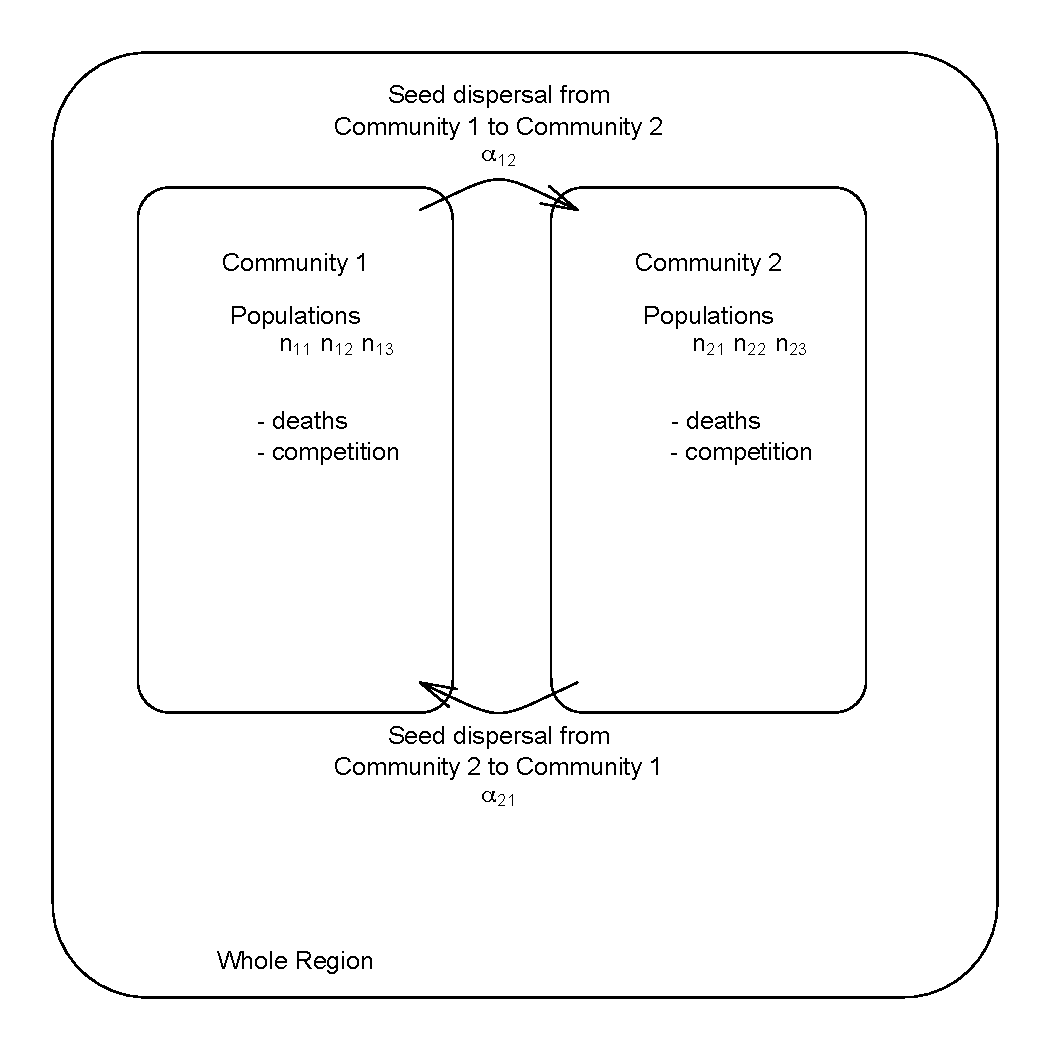
\includegraphics[width=4.5in]{schematic.pdf}
\caption[The metapopulation framework]{\textbf{The metapopulation framework:} We consider a region composed of two separated communities. Within each communities, populations of each of the three species may persist, where individuals die and seeds produced by the remaining adults compete over the resulting gap. Seeds can disperse between patches, a seed will move from community $k$ to community $l$ with probability $\alpha_{k,l}$ when a gap appears in the canopy.}
\label{fig:schematic}
\end{center}
\end{figure}

The effects of dispersal limitation and localised disturbance on the results are also examined while treating spatial patterns implicitly, using a metapopulation sturcture. The system is divided into two smaller patches $N_1,N_2$ which each may experience different disturbance regimes. For example, the community $N_1$ may be protected from disturbance by some geographical feature, but which may also limit the connectedness of the two communities. Within each of these patches, dynamics occur as described above, as individuals die and species compete for opened sites locally. It is within these two patches that we measure local, or $\alpha$, species richness. We denote the populations of species $i$ in community $k$ by $n_{k,i}$, with patch 1 containing the populations $n_{1,1}, n_{1,2}, n_{1,3}$ while the second community consists of populations $n_{2,1}, n_{2,2}, n_{2,3}$, as shown in Figure~\ref{fig:schematic}.

Dispersal between patches is also considered. Each seed produced during a time step is assigned a probability of being dispersed between the two patches. This probability is denoted $\alpha_{k,l}$, the probability of a seed in community $k$ dispersing to the other patch, containing community $l$, as denoted by the arrows in Figure~\ref{fig:schematic}. The expected number of species $i$ seeds competing for a gap created in community $k$ is given by $(1-\alpha_{k,l})s_in_{k,i} + \alpha_{l,k}s_in_{l,i}$. A proportion $\alpha_{l,k}$ of seeds produced in community $l$ will disperse into the community $k$, while $\alpha_{k,l}$ of the seeds produced by species $i$ individuals in community $k$ leave the patch via dispersal, leaving a proportion $1-\alpha_{k,l}$ to compete over the gap Therefore, the probabilities of each species claiming a site that is emptied in community $k$ are given by
\begin{align}
\label{c1patched}
c_1(S_1,S_2,S_3)=&\frac{S_1 \exp(-x_{1,2}S_2/N)\exp(-x_{1,3}S_3/N)}{\sum_{k=1}^3 S_k},\\
c_2(n_1,n_2,n_3)=&\frac{S_1(1-\exp(-x_{1,2}S_2/N)\exp(-x_{1,3}S_3/N))}{\sum_{k=1}^3 S_k}\frac{S_2\exp(-x_{2,3}S_3/N)}{S_2+S_3} \notag \\
&+\frac{S_2\exp(-x_{2,3}S_3/N)}{\sum_{k=1}^3 S_k} \\
c_3(S_1,S_2,S_3)=&1-c_1(S_1,S_2,S_3)-c_2(S_1,S_2,S_3)
\end{align}
where $S_i$ is the number of species $i$ seeds present in the community after randomised dispersal has taken place.

We also measure $\gamma$ diversity in the metapopulation model, by combining the populations of both patches.

\section{Results}
\subsection{Single patch environment with no disturbance}
\textbf{First, we consider the case with a single community in a single patch. We examine the persistence of the three species over a range of $x-$space in the absence of disturbance}. Since $x_{2,3}=x_{1,3}-x_{1,2}$ from the definition of $x_{i,j}$, we can consider different combinations of 
$x_{1,2}$ and $x_{1,3}$ to get a complete picture of the parameter space for growth rates for the species. Using fixed seed numbers $s_1=500,s_2=100,s_3=20$ we can examine the behaviour of the system under many different circumstances by simply varying the $x_{i,j}$ (See Figure~\ref{xregions}). \textbf{We simulate times series of population dynamics for a broad range of $x_{1,2}$ and $x_{1,3}$ and examine the impact on community structure when} moving between regions of $x-$space as shown in Figure~\ref{xregions}, while also examining the effects of the initial populations on the outcome. We run simulations that vary initial populations by 100 , considering all combinations of $n_1,n_2,n_3$ that (a) Satisfy that each species begins with $100q$ individuals present for $q \in \{1,2,3,4,5,6,7,8\}$ and (b) the three populations sum to $N=1000$. 
\begin{figure}[htbp]
\begin{center}
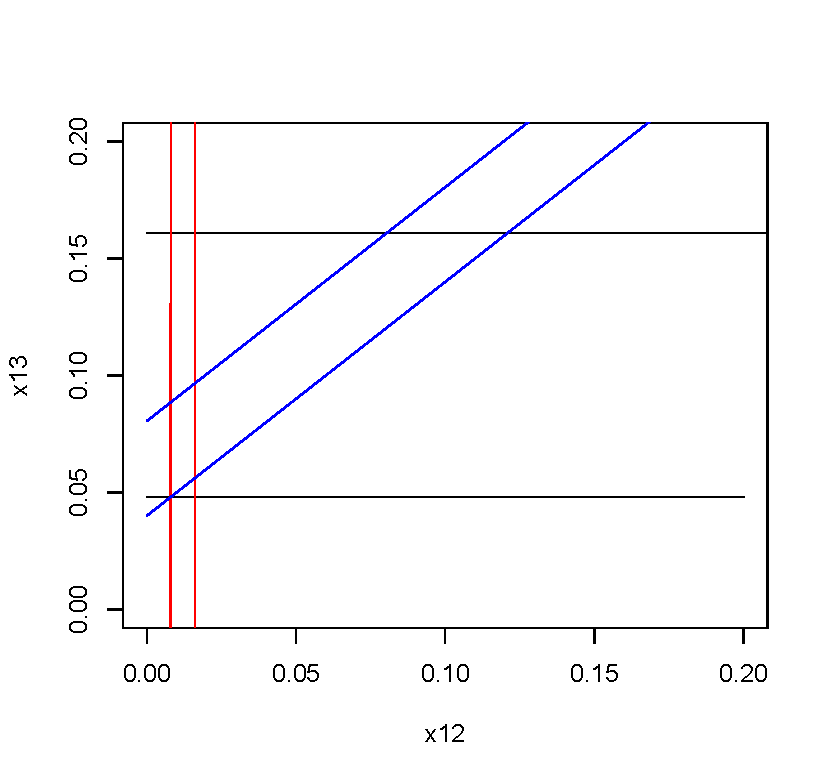
\includegraphics[width=4in]{3dxchoices.pdf}
\caption[The different regions of $x-$space]{\textbf{The different regions of $x-$space:} The regions of $x-$space that give coexistence for the 3 possible species pairs. Species 1 and 2 can coexist between the red, vertical lines. Species 1 and 3 coexist between the black horizontal lines, while species 2 and 3 can coexist between the blue, diagonal lines. Seed numbers used are $s_1=500,s_2=100,s_3=20$.}
\label{xregions}
\end{center}
\end{figure}
When species 3 dominates both species 1 and 2 (top left), it dominates the three species environment as expected, driving both other species to extinction. Similarly, when species 1 excludes each of the two less fecund species, it also dominates in the three species case. However, when species 2 dominates both the more fecund species 1 and the faster growing species 3 in pairwise competition (the right hand side region of Figure\ref{xregions}), there is an element of founder control. When species 3 excludes species 1 in pairwise competition, the outcome is driven by the initial populations. If species 2 is initially at a much lower population than species 3, species 3 will persist in monoculture, while if the initial population of species 2 is sufficiently high, it will exclude both the fecund species 1 and the fast growing species 3. Similarly, when species 1 excludes species 3, if the species 2 population in initially low, then species 1 will dominate the environment, while for higher initial populations species 2 dominates. When species 1 and 3 can coexist but are both excluded by species 2, in the three species case, it is necessary for species 2 to have a high initial population in order to persist, in which case it will exclude both other species. However, if species 2 has a lower initial population, then species 1 and species 3 will coexist together and exclude the generalist species 2.

A similar pattern is observed when species 2 can coexist alongside one of the other species, yet excludes the third species. When species 2 and 3 can persist together, and species 2 excludes species 1, then founder control again occurs. If $n_2(0)$ is sufficiently high, species 1 will be driven to extinction and the species 2 and 3 coalition will persist, but if the initial population is too low, species 2 will be excluded, and the outcome of the model simulations is determined by the two species interactions between the fecund species 1 and the rapidly growing species 3. Similarly, when species 1 and 2 can coexist, and species 2 excludes species 3, a sufficiently low initial population will instead result in species 2 being excluded, and the outcome is determined by the interactions of species 1 and 3, while a high initial population will exclude species 3, allowing the species 1 and 2 coalition to thrive.

In all other cases, species 2 is excluded regardless of initial populations, and the behaviour of the model is determined by the two species analysis of Chapter~2 applied to species 1 and 3.

\subsection{Single patch environment with disturbance affecting all species equally} \label{ss:homo}
When setting $I_i=I$ for all $i \in \{1,2,3\}$, such that disturbance affects all species equally, the response of the system to disturbance is determined by the non-disturbance behaviour outlined above. We assume frequency is sufficiently high to not have a significant effect (see Chapter 2) and consider the impact of increasing disturbance intensity. If species 1 excludes both other species in a homogeneous environment, the only effect disturbance has is to accelerate this. When species 1 coexists with either species 2 or species 3 in the homogeneous environment, then as disturbance intensity increases, it will exclude the less fecund competing species, although they will still coexist at low intensity. When either species 2 or species 3 exists in monoculture in a disturbance free environment, as intensity is increased they will coexist along side species 1. When intensity is increased further, species 1 will exclude the less fecund, rapid growth species. When species 2 and 3 coexist in the disturbance free case, intensity can cause different community structures. At low intensity, species 2 and 3 will continue to exclude species 1. As intensity increases, the generalist species 2 will exclude both the less fecund species 3 and the poor local competitor species 1. Increase intensity further, and species 1 and 2 will coexist while species 3 is excluded, while at very high intensities, species 1 will exclude both species 2 and 3.

\subsection{Single patch environment with a defence specialist}
In most cases, the generalist species 2 is outcompeted by the two specialists eroding some of its niche from either side. Does a specialisation in defence against disturbance allow species 2 to survive alongside the growth and colonisation specialists? We set $I_1=I_3=yI_2$, and vary $y>1$ so examine the effects of defence specialism by species 2. We find that increasing the disturbance intensity will initially just repeat the anticipated behaviour when all 3 species suffer the same intensity. For $y$ sufficiently close to 1 ($y=1.1$), this will continue and the `expected' behaviour will occur. However, for larger $y$ ($y=2$ and $y=10$), as intensity is increased further, the advantage in disturbance survival for species 2 becomes the dominant force behind the dynamics, and both species 1 and 3 are excluded, with species 2 existing in monoculture. We conclude that resistance to disturbance mortality of the generalist cannot increase biodiversity along a fecundity-growth trade-off.

\subsection{Metapopulation model}
\textbf{We now consider the metapopulation model described in Section~\ref{metapopmodel}. When disturbance regimes do not differ between patches, coexistence of all three species at a region-wide scale cannot occur for any level of between patch migration $\alpha_{1,2},\alpha_{2,1}>0$ (e.g. Figure~\ref{fig:regions}(a) and Figure~\ref{wholereg}(a)). This is the case even when initial absence of a species from a patch will result in region wide exclusion of one of the three species.} We therefore focus on a region of trait space where any of the three species can persist at differing levels of intensity for high frequency disturbances. From \ref{ss:homo} we thus choose a region of $x-$space where the result in a homogeneous environment is that the strong local competitor species 3 and the generalist species 2 coexist, while excluding the fecund species 1. One such choice of parameters is given in Table~\ref{tab:paras}, which we use henceforth, \textbf{although the results do not qualitatively change for other parameters where species 2 and 3 exclude the fecund species 1 when disturbance is absent}. Note that for these chosen parameters, species 2 will be excluded in the non-disturbance case when it's initial population is too low. We select initial populations whereby species 2 has a sufficiently high population to persist in the environment ($n_{i,2}(0)=0.5N_i,n_{i,1}(0)=0.3N_i$). Then species 1 is present when disturbance frequency is high and for intensities $I\geq0.75$, which species 3 persists in the system for low intensities $I\leq 0.15$. Meanwhile, species 2 will persist for all intensities $I\leq 0.8$.
\begin{table}[htdp]
\begin{center}
\begin{tabular}{|c|c|} \hline
Parameter & Value\\ \hline
$s_1$&500\\
$s_2$&100\\
$s_3$&20\\
$x_{1,2}$&0.05\\
$x_{1,3}$&0.1\\
$N$&2000\\ \hline
\end{tabular}
\end{center}
\caption[Parameters used for examination of patchy disturbance]{Parameters used for examination of patchy disturbance using metapopulation model}
\label{tab:paras}
\end{table}
We assume that community 1 (size $N_1$) does not experience any disturbance (although simulations give qualitatively similar results providing the disturbance regime in this community is of sufficiently low intensity to allow the persistence of the least fecund species). For example, the first community may be a nature reserve where logging is prohibited, while the second community experiences disturbance via logging. Thus, when entirely unconnected to the second community ($\alpha_{1,2}=\alpha{2,1}=0$), species 2 and 3 will persist.

When disturbance pressure varies between patches, regional coexistence is possible (Figure~\ref{wholereg}(b) and (c)). As community 1 is protected from disturbance, the outcome of the dynamics in this patch is coexistence of the two best local competitors, species 2 and 3, while the fecund species 1 is excluded. As disturbance intensity is increased in the community in patch 2, however, the least fecund species 3 is excluded. For some disturbance intensities ($0.75\leq I\leq0.85$ with the current parameters), species 1 and 2 will coexistence in this community (Figure~\ref{fig:regions}(b) shows $I=0.8, T_D=5$), while for extremely high intensities, species 1 will live in monoculture, having excluded both competitors. When species 1 is present in community two, the whole region will exhibit three species coexistence (Figure~\ref{wholereg}(b)).

As connectedness of the two communities ($\alpha_{1,2}, \alpha_{2,1}$) is increased, with seed dispersal or alternative processes (e.g. the movement of adult plants by horticulturists) linking the two sites, it becomes possible for the regional processes allowing multi-species coexistence to inflate local biodiversity. As shown in Figure~\ref{fig:regions}(c), the migration of seeds creates coexistence of three species in the disturbed community 2, as the refuge community 1 has much fewer gaps created. This makes it more difficult for the excluded, fecund, species to invade. In the disturbed community, however, there are a larger number of gaps are created when a disturbance occurs, thus increasing the probability of settlement by the poor coloniser (species 3), which would be excluded should there be no immigration from the refuge. At a regional scale, low levels of inter-patch dispersal do not qualitatively affect the result, that of three species coexistence in the region (Figure~\ref{wholereg}(b) and (c)). Note that if dispersal between patches is likely (high $\alpha_{k,l}$), then the population behaves as would be expected for the single patch model considered above, and species 1 will be excluded. In this scenario, the refuge in community 1 serves to allow persistence of the less fecund species 3 for higher intensities than the single patch model, but three species coexistence cannot occur. 

\begin{figure}[htbp]
\begin{center}
\begin{tabular}{ccc}
(a)&&\\
&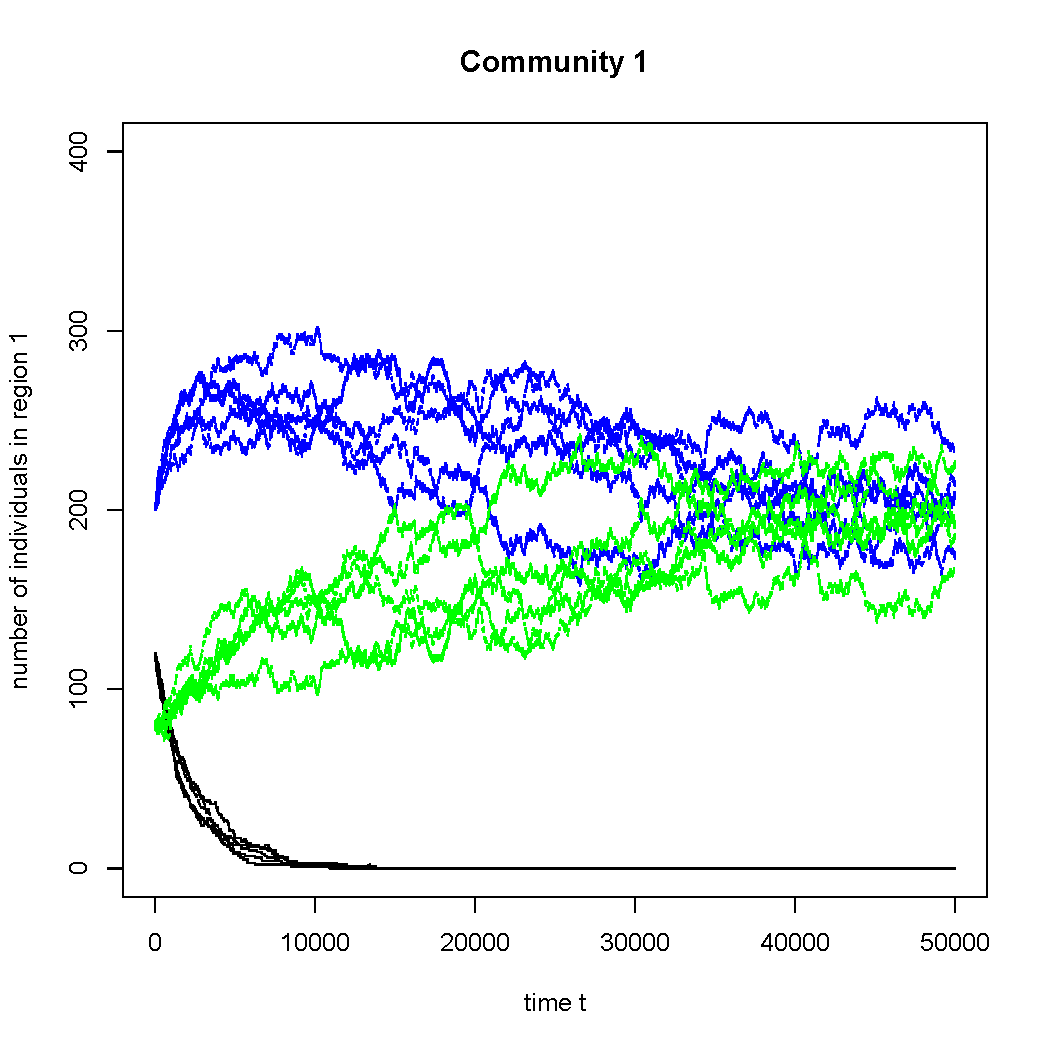
\includegraphics[width=2in]{region1nodist} &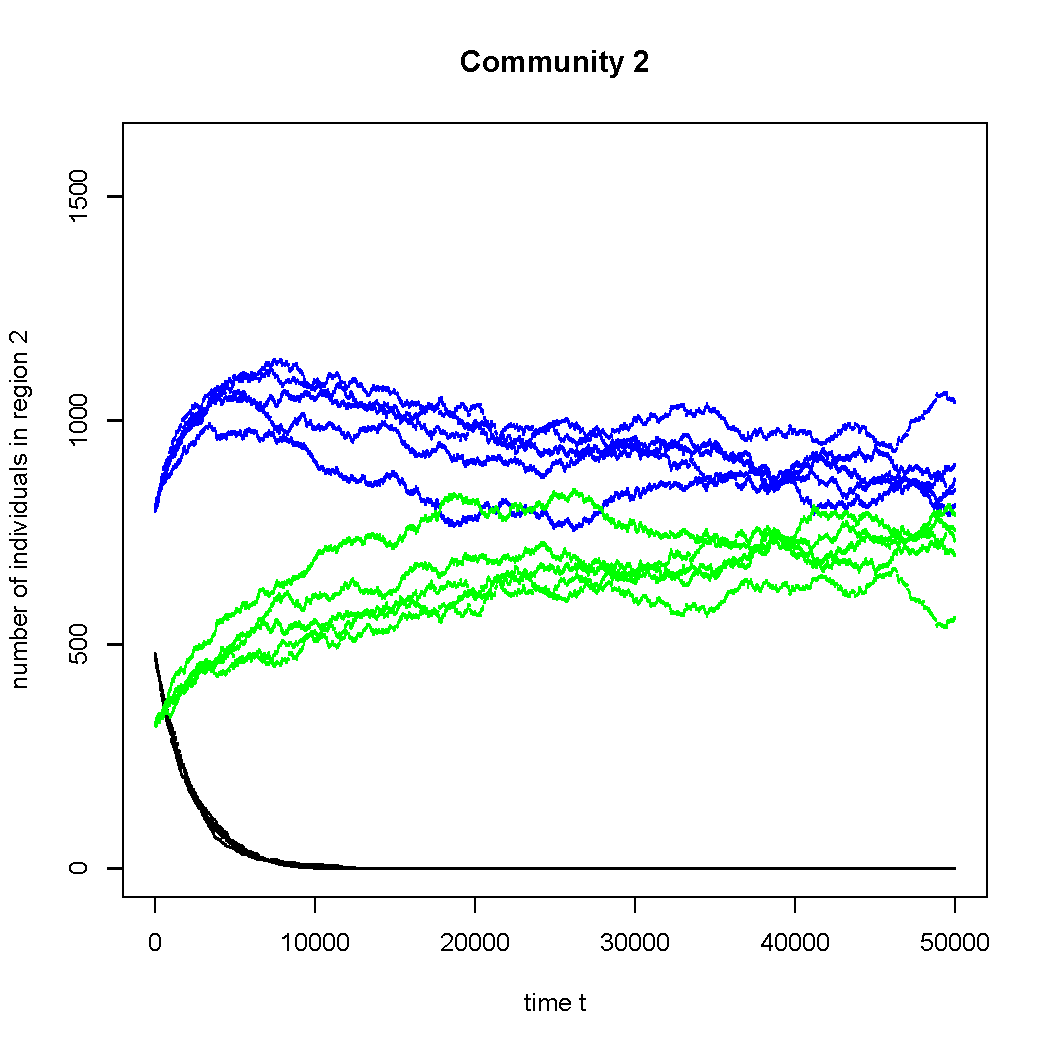
\includegraphics[width=2in]{region2nodist}\\
(b)&&\\
&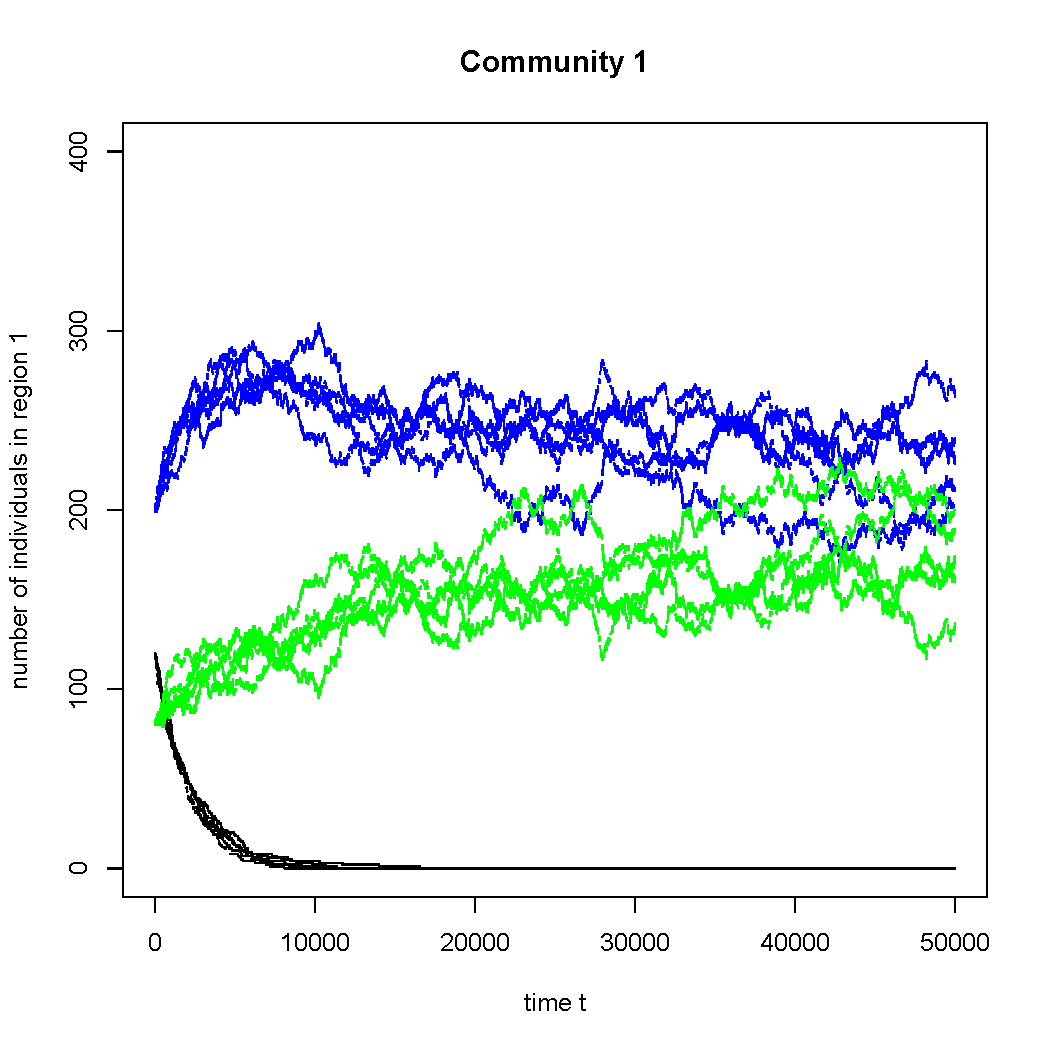
\includegraphics[width=2in]{region1distnotmixed} &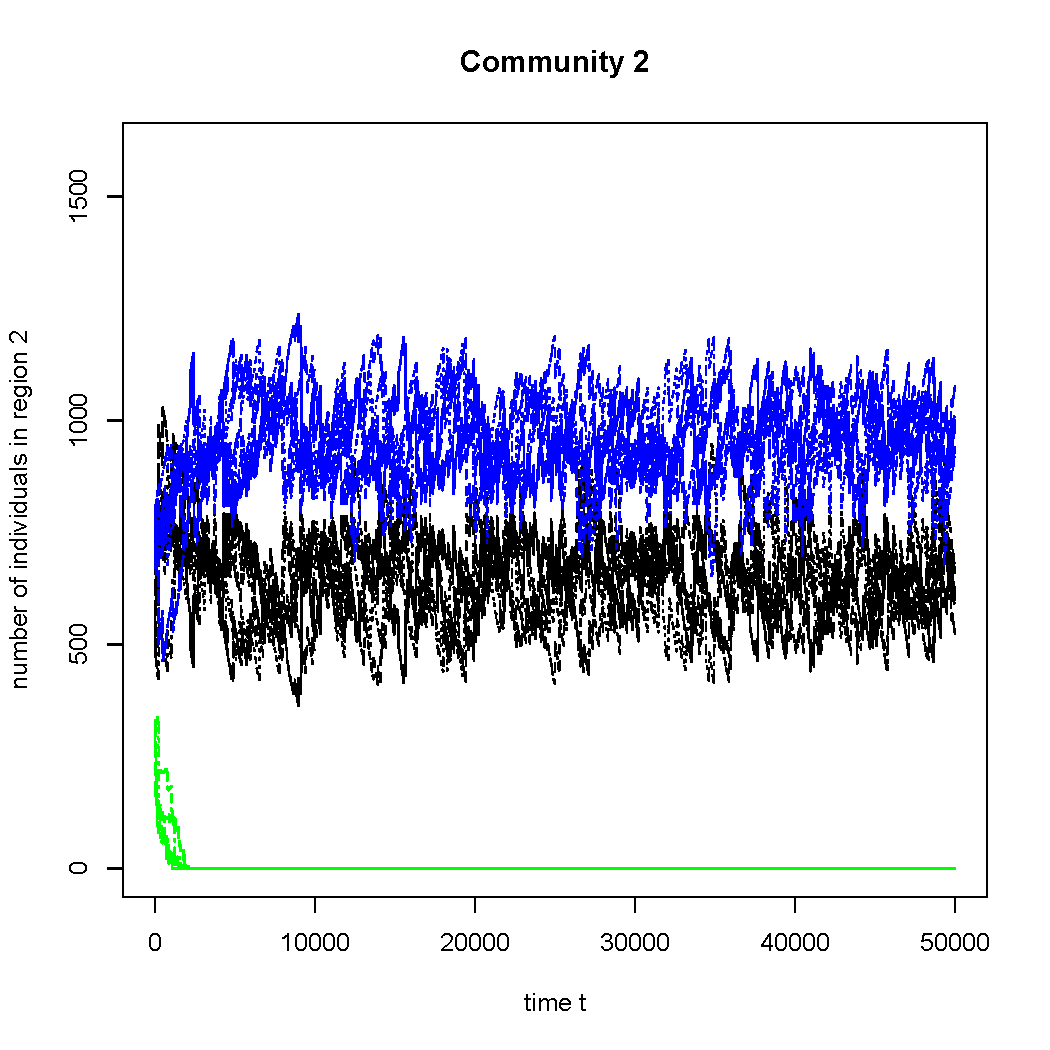
\includegraphics[width=2in]{region2distnotmixed}\\
(c)&&\\
&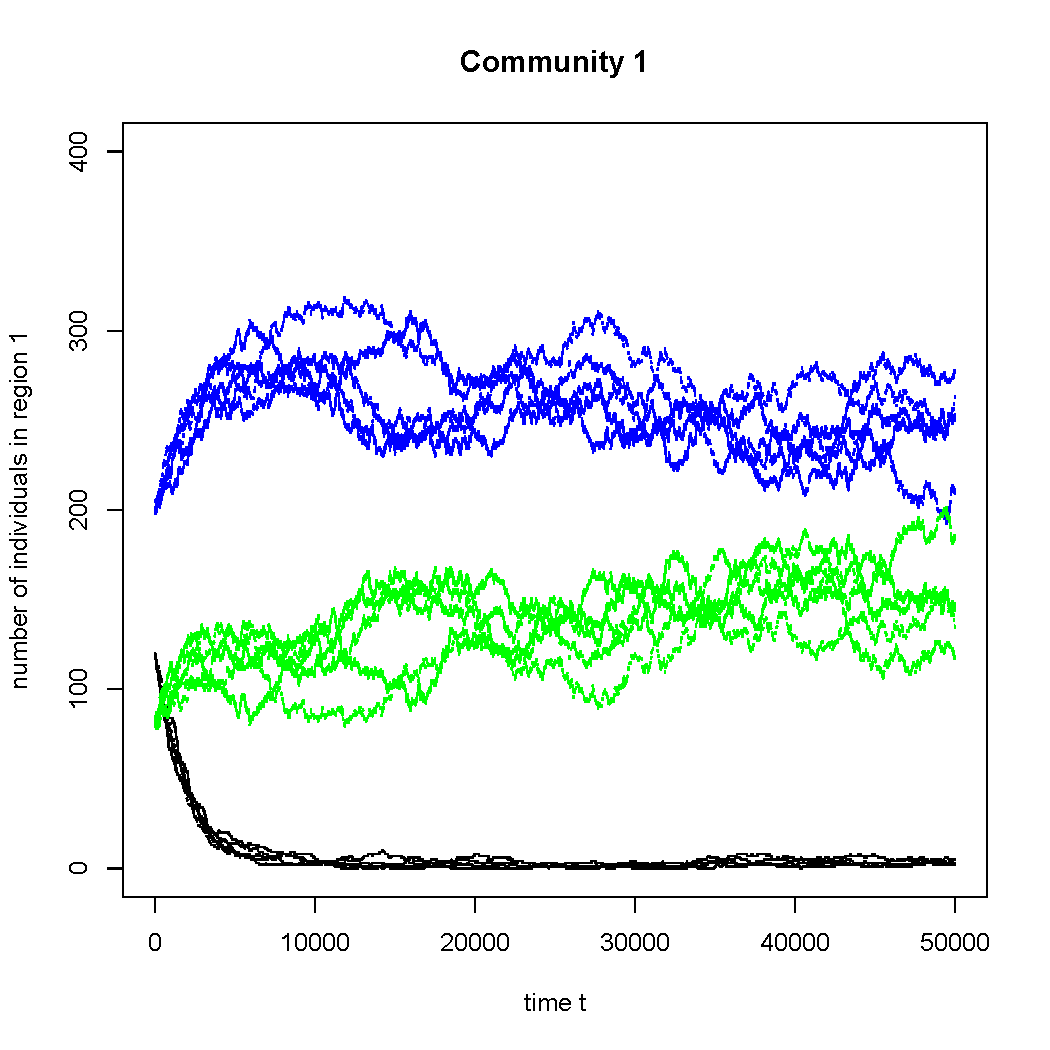
\includegraphics[width=2in]{region1distandmixed} &\includegraphics[width=2in]{region2distandmixed}
\end{tabular}
\caption[Effects of disturbance and dispersal on two community patches]{\textbf{Effects of disturbance and dispersal on two community patches:} How the two patch metapopulation model responds to local disturbance and dispersal between sites. (a) When disturbance regimes are the same in both communities, the dynamics mirror each other. With the parameters in Table~\ref{tab:paras} and no disturbance, the most fecund species 1 is excluded in both patches. (b) When disturbance occurs in community 2, but no seeds disperse between communities, the outcome of community 1 is unaffected, species 2 and 3 are both present. In community 2, when $T_D=5, I=0.8$, the least fecund species 3 is excluded, and species 2 coexists alongside species 1. (c) When disturbance occurs in patch 2 and there is dispersal between sites, the outcome in community one, without disturbance, is largely unaffected, although species 1 does occasionally gain some sites by dispersing seeds from community 2. However, these periods are brief. In community two, dispersal of the least fecund species 3 can allow it to persist alongside the two species that would exclude it without dispersal. The probability of a seed moving between patches in these simulations is 0.05. Plot shows 5 simulations of each scenario for 50000 time steps. Black represents species 1, species 2 is represented by blue, while species three populations are tracked by the green lines.}
\label{fig:regions}
\end{center}
\end{figure}

\begin{figure}[htbp]
\begin{center}
\begin{tabular}{cc}
(a)&\\
&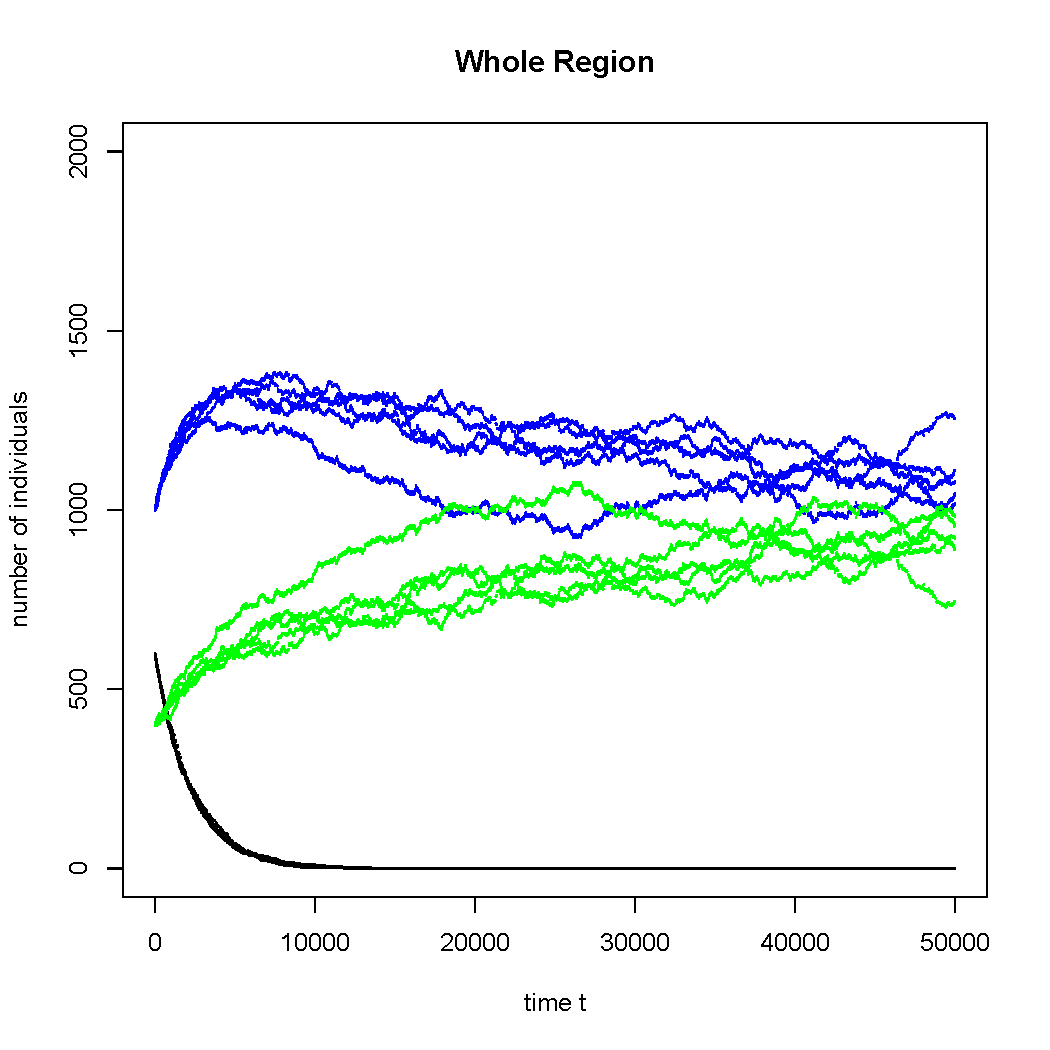
\includegraphics[width=2in]{wholeregionnodist} \\
(b)&\\
&\includegraphics[width=2in]{wholeregiondistnotmixed} \\
(c)&\\
&\includegraphics[width=2in]{wholeregiondistandmixed} 
\end{tabular}
\caption[Effects of disturbance and dispersal on regional $\gamma$ diversity]{\textbf{Effects of disturbance and dispersal on regional $\gamma$ diversity:} How the two patch metapopulation model populations appear as viewed across the whole region when responding to local disturbance and dispersal between sites. (a) When disturbance regimes are the same in both communities, only two species persist in the region. (b) When disturbance occurs in community 2, but no seeds disperse between communities, all three species persist in the environment. Species 2 and 3 are present in community 1, while species 1 and 2 are present in community 2, exposed to disturbance (Figure~\ref{fig:regions}) (c) When disturbance occurs in patch 2 and there is dispersal between sites, the regional populations are largely unaffected by low levels of seed dispersal, and all three species persist at similar population levels to the case where dispersal does not occur. Plot shows 5 simulations of each scenario for 50000 time steps. Black represents species 1, species 2 is represented by blue, while species three populations are tracked by the green lines.}
\label{wholereg}
\end{center}
\end{figure}


\subsubsection{Effects of varied refuge patch size}
As the proportion of the forest protected from disturbance $N_1/N$ is varied, we find that the range of connectedness ($\alpha_{1,2}=\alpha_{2,1}=\alpha$, which is varied in increments of 0.05) for which all three species can persist at a given intensity is maximised at an intermediate value of $N_1/N$, as shown in Figure~\ref{fig:alpharange}. Only refuges below a certain proportion of the community can support all three species when there is mixing between the two communities. When the refuge becomes large, and the unprotected area small, the effect is to reduce the population of the fecund species 1. As this species requires the space created by disturbance events to survive in the environment, the limited amount of space created by a disturbance, combined with the high mortality of species one in this part of the environment, results in the extinction of the most fecund species.

\begin{figure}[ht]
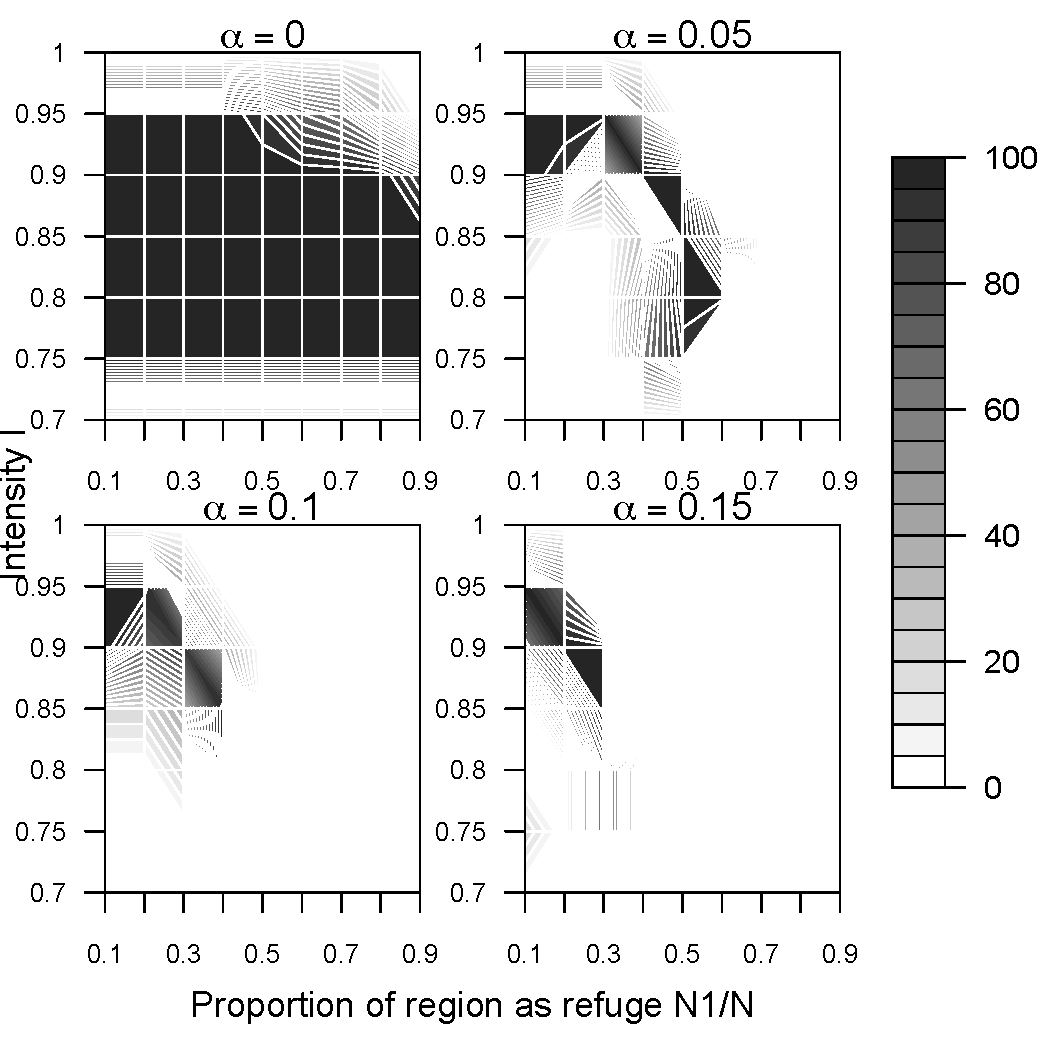
\includegraphics[width=4.5in]{refugesize.pdf}
\caption[Effects of refuge size on multi-species coexistence]{The effects of varied refuge size of the likelihood of three species coexistence. Shaded areas represent the coexistence of all three species regionally after 50000 event time-steps. When $\alpha>0$, coexistence is only possible for relatively small refuges, while when the protected community is significantly larger than the disturbed area, coexistence is not possible for any non-zero level of cross-colonisation.}
\label{fig:alpharange}
\end{figure}

\section{Discussion}
Understanding the ways in which species diversity is generated and supported is a crucial problem in ecology, with great relevance for conservation practices. The role of environmental variability, such as disturbance events, is an important area of consideration. This is becoming more crucial, as climate change is predicted to have dramatic impacts on the frequency and intensity of such events \citep[e.g.][]{webster2005changes}. In this chapter, the possibility of multi-species ($n>2$) coexistence is examined in an environment defined by the disturbance regimes. Within this model framework, with species differing only along a fecundity-growth trade-off, it is only possible for more than two species to coexist if the environment has some spatial heterogeneity combined with the temporal heterogeneity of disturbance events. In that case, the existence of a protected community that does not experience disturbances that effect the neighbouring community (for example, a nature reserve where logging is prohibited, or a no-take zone alongside a heavily trawled region of ocean) can promote regional coexistence of more than two species. In addition, if limited dispersal occurs between the two communities, it is possible that the local species richness outside the protected community will also be increased, without observing a corresponding increase within the reserve. This may have important consequences for the placement and management of nature reserves, which often seek to cover environmental regions that support all species \citep[e.g.][]{margules1988selecting,scott2001nature}.

The coexistence of three species within this model framework appears to be more robust when the protected area, or refuge, is relatively small in comparison with the neighbouring environment. Small protected areas in large areas experiencing disturbance can enable the region-wide support of multiple species for much higher levels of dispersal between the disturbed and protected communities. \textbf{That small reserves maximise regional coexistence concurs }with the findings of \cite{lasky2013reserve}, who find $\gamma$ diversity is maximised for small reserves. These results indicate that under some circumstances, where disturbance comes in the form of human pressure such as logging, it may be possible that careful management of the system would allow for a large area to be logged, while the region continues to support a large number of species.
\cite{lasky2013reserve} find that large reserves have higher $\alpha$ diversity, we find that there is no relationship between the number of species present within the reserve, \textbf{although this may be due to the small number of species in our model}. Instead, the boost in $\gamma$ diversity gained by small reserves is triggered by an increase in an increase in species richness in the unprotected community neighbouring the reserve.

However, it is only possible for two species to coexist when the environment is considered as a single patch, with no spatial heterogeneity, either with or without disturbance events. This result in the non-disturbance case, where the environment is both spatially and temporally homogeneous, lends support to previous predictions that coexistence is unlikely when species face a trade-off affecting per capita reproduction, such as the fecundity-growth trade-off considered here \citep{egas2004evolution}.
 However, these results appear to conflict with empirical data, where coexistence of generalists and specialists is common \citep[e.g.][]{morris1996coexistence,bonesi2004differential}. 
 
 Further, if all three species are present in a single, isolated patch at $t=0$, then the generalist species (here species 2) can only persist in the environment when the initial population is sufficiently high, in both environments with and without disturbance. This result is in contrast to those of both \cite{marvier2004habitat} and \cite{nagelkerke2013coexistence}, who find short term disturbances tend to favour generalist species. The difference in our results may be a consequence of the assumption by Marvier et al. that species that spread tend to be generalists, while the model presented here assumes that the more fecund species is the most successful coloniser, and therefore is the species to benefit from the creation of a large number of empty sites. A second assumption here is that all species can survive in isolation across the entire disturbance gradient (providing $I_i<1$), and the niche segregation into fecundity specialist and light competition specialist is dependent on the specific species composition of the region. In contrast, both the model of  \cite{marvier2004habitat} and that of \cite{nagelkerke2013coexistence} assume specialist species can only survive in certain habitat types, independent of the presence or absence of a competing species. The current model also predicts that allowing the generalist species an advantage in disturbance defence does not permit multi-species coexistence. This may be because an increase in fecundity and an increase in defence against disturbance effectively operate along the same environmental axis, both increasing fitness within a disturbance event.
 
 The results presented here emphasise that disturbance can be a key contributor to species richness, and that considering different factors that make up disturbance, including spatial structure, can be crucial in predicting how a community will respond to disturbance pressure (see also Chapter~2). This chapter examines the effects of disturbance extent, where a portion of the environment is protected, either naturally or by governmental policy, and demonstrate that this can help promote species richness at \textbf{different spatial scales, as $\gamma$ diversity is increased by protected communities, and the local $\alpha$ diversity can also be boosted in one patch}. Perhaps counter-intuitively, it is possible to observe an increase in local diversity outside the refuge from disturbance, while no such increase is observed within the protected area. This suggests that  future empirical work should not only focus on events within the protected areas \citep[e.g.][]{pyvsek2002plant,kitchner1982predictors}, but must also consider the effects of introducing the reserve on neighbouring communities that remain unprotected.
 